\section{Use case diagram}
Here we include a diagram which contains all the use cases that are relevant for this system.
\begin{landscape}
\includepdf[scale=0.95,angle=90]{pdfs/use_case.pdf}
\end{landscape}


\section{Class diagram}
Here we include sketch of a possible class diagram for the system. 

It should be noted that this diagram is intended to be used as a preliminary draft for further analysis in the design phase, and that it doesn't fully represent the final class infrastructure the shipped system will be based upon.

Furthermore, this diagram only covers the classes that are present in the central system and doesn't include the structure of the mobile applications and of the web applications.

\begin{landscape}
%\includegraphics[width=850pt,keepaspectratio]{pdfs/class_diagram.pdf}
%\includepdf{pdfs/class_diagram.pdf}
\includepdf[scale=0.95,angle=90]{pdfs/class_diagram.pdf}
\end{landscape}


\section{Activity diagrams}
\subsection{Request a taxi}
\begin{figure}[H]
\centering
\makebox[\columnwidth]{\includegraphics[width=\textwidth,keepaspectratio]{pdfs/01_call_taxi.pdf}}
\end{figure}


\subsection{Place a taxi reservation} %
\begin{figure}[H]
\centering
\makebox[\columnwidth]{\includegraphics[width=300pt,keepaspectratio]{pdfs/02_reserve_taxi.pdf}}
\end{figure}\nopagebreak



\subsection{Reservation allocation} %
\begin{figure}[H]
\centering
\makebox[\columnwidth]{\includegraphics[width=300pt,keepaspectratio]{pdfs/03_allocate_taxi.pdf}}
\end{figure}


\subsection{Confirm a ride has ended}
\begin{figure}[H]
\centering
\makebox[\columnwidth]{\includegraphics[width=300pt,keepaspectratio]{pdfs/04_end_ride.pdf}}
\end{figure}


\subsection{Set a driver's status to unavailable}
\begin{figure}[H]
\centering
\makebox[\columnwidth]{\includegraphics[width=280pt,keepaspectratio]{pdfs/05_unavailable.pdf}}
\end{figure}


\section{Sequence diagram}
Here we include a sequence diagram for the “request a taxi” operation.

For the sake of simplicity and readability, only the main flow of execution has been included in this diagram. Alternative flows of executions, such as those related to unexpected situations or exceptions, are not covered.

\begin{landscape}
\includepdf[scale=0.95,angle=90]{pdfs/sequence.pdf}%
\end{landscape}


\section{State chart diagram}
This state chart models the possible states in which a taxi can be inside the system and the transitions between them.

It should be noted that the states the system recognizes are not mapped one-to-one to all the possible states a taxi can be in. 

In particular, the taxi transition from the inside to the outside of the city and viceversa is not modeled if the taxi is performing a ride or if he's unavailable; that means that the status of the taxi will not change when crossing the border if the taxi is not in the “available” status. 

This is not a limitation for the system: in fact, we don't need to know whether a taxi is inside or outside the city if he's performing a ride or if he's unavailable, because in either case he would not be able to receive requests anyway.

\begin{figure}[H]
\centering
\makebox[\columnwidth]{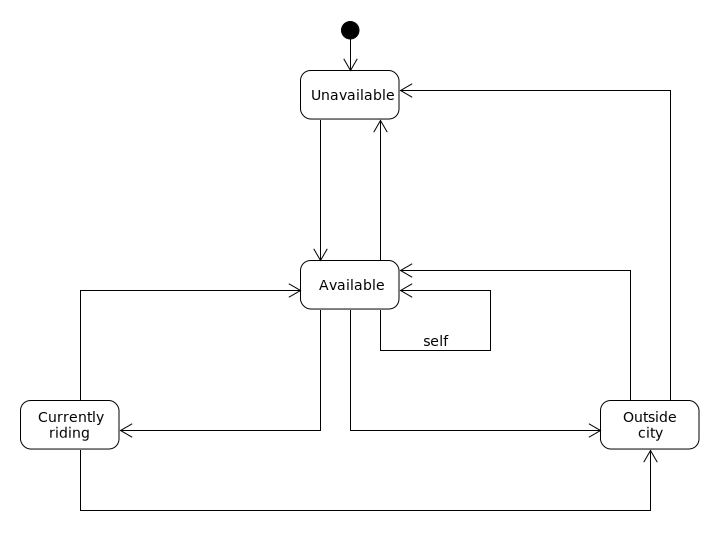
\includegraphics[width=350pt,keepaspectratio]{pdfs/statechart.pdf}}
\end{figure}
\pagebreak

